% THIS IS AN EXAMPLE DOCUMENT FOR VLDB 2010
% based on ACM SIGPROC-SP.TEX VERSION 2.7
% Modified by  Gerald Weber <gerald@cs.auckland.ac.nz>


% This example *does* use the .bib file (from which the .bbl file
% is produced). REMEMBER HOWEVER: After having produced the .bbl file,
% and prior to final submission, you need to 'insert'  your .bbl file into
% your source .tex file so as to provide ONE 'self-contained' source file.

\documentclass{vldb}
\usepackage{graphicx}
\usepackage{balance}  % for  \balance command ON LAST PAGE  (only there!)


\begin{document}

% ****************** TITLE ****************************************

\title{Using Deep Learning to Perform Fuzzy Joins}

% possible, but not really needed or used for PVLDB:
%\subtitle{[Extended Abstract]
%\titlenote{A full version of this paper is available as\textit{Author's Guide to Preparing ACM SIG Proceedings Using \LaTeX$2_\epsilon$\ and BibTeX} at \texttt{www.acm.org/eaddress.htm}}}

% ****************** AUTHORS **************************************

% You need the command \numberofauthors to handle the 'placement
% and alignment' of the authors beneath the title.
%
% For aesthetic reasons, we recommend 'three authors at a time'
% i.e. three 'name/affiliation blocks' be placed beneath the title.
%
% NOTE: You are NOT restricted in how many 'rows' of
% "name/affiliations" may appear. We just ask that you restrict
% the number of 'columns' to three.
%
% Because of the available 'opening page real-estate'
% we ask you to refrain from putting more than six authors
% (two rows with three columns) beneath the article title.
% More than six makes the first-page appear very cluttered indeed.
%
% Use the \alignauthor commands to handle the names
% and affiliations for an 'aesthetic maximum' of six authors.
% Add names, affiliations, addresses for
% the seventh etc. author(s) as the argument for the
% \additionalauthors command.
% These 'additional authors' will be output/set for you
% without further effort on your part as the last section in
% the body of your article BEFORE References or any Appendices.

\numberofauthors{3} %  in this sample file, there are a *total*
% of EIGHT authors. SIX appear on the 'first-page' (for formatting
% reasons) and the remaining two appear in the \additionalauthors section.

\author{
% You can go ahead and credit any number of authors here,
% e.g. one 'row of three' or two rows (consisting of one row of three
% and a second row of one, two or three).
%
% The command \alignauthor (no curly braces needed) should
% precede each author name, affiliation/snail-mail address and
% e-mail address. Additionally, tag each line of
% affiliation/address with \affaddr, and tag the
% e-mail address with \email.
%
% 1st. author
\alignauthor Abraham Judah Gale \\
% \titlenote{Dr.~Trovato insisted his name be first.}\\
       \affaddr{Thesis Submitted to}\\
       \affaddr{Yeshiva University}\\
  %     \affaddr{Wallamaloo, New Zealand}\\
       \email{yehuda.gale@gmail.com}
% 2nd. author
\alignauthor
Kavitha Srinivas \\
% \titlenote{The secretary disavows
% any knowledge of this author's actions.}\\
     \affaddr{Advisor}\\
       \affaddr{Rivet Labs}\\
 %      \affaddr{Dublin, Ohio 43017-6221}\\
       \email{Kavitha@rivetlabs.io}
% 3rd. author
\alignauthor Judah Diament\\
       \affaddr{Advisor}\\
       \affaddr{Yeshiva University }\\
       \email{diament@yu.edu}
}
% There's nothing stopping you putting the seventh, eighth, etc.
% author on the opening page (as the 'third row') but we ask,
% for aesthetic reasons that you place these 'additional authors'
% in the \additional authors block, viz.
% \additionalauthors{Additional authors: John Smith (The Th{\o}rv\"{a}ld Group,
% email: {\texttt{jsmith@affiliation.org}}) and Julius P.~Kumquat
% (The Kumquat Consortium, email: {\small \texttt{jpkumquat@consortium.net}})}
% \date{30 July 1999}
% Just remember to make sure that the TOTAL number of authors
% is the number that will appear on the first page PLUS the
% number that will appear in the \additionalauthors section.


\maketitle



\section{Introduction}

Joining two datasets is a key step in preparing the data for subsequent operations such as performing business analytics, building predictive models etc.  Data management systems have largely focussed solely on equi-joins, which is based on exact equality of strings or numeric values.  However, in many circumstances, exact equality is inadequate because the same entity may in many cases be expressed with slight variations of the same name, as shown in Figure~\ref{table-example} (e.g., \textit{Douglas Adams} and \textit{Douglas Noel Adams}).  Although Figure~\ref{table-example} illustrates the problem for people's names, the same problem occurs for other entity types, such as company names, addresses, states in countries, and countries.

One common technique to automating joins of the sort described in Figure \ref{table-example} is string matching.  String matching approaches use variants of string similarity measures such as edit-distance, Jaro-Winkler and TF-IDF (e.g., \cite{Cohen2003}) to perform matching.  Typically to scale the problem to a large number of rows in each table, a filtering or blocking strategy is used to reduce the number of pairs to be considered for string matching.  For instance, prefix, string length, or suffix based filtering are often applied to the strings in the two tables to identify potentially joinable pairs that need to be matched.  For the examples shown in Figure~\ref{table-example}, the prefix filtering step will ensure that \textit{Douglas Adams} will be compared only with \textit{Douglas Noel Adams} and \textit{Doug C. Engelbart} to determine their string similarity, assuming the prefix used for filtering is \textit{Doug}.  

More recently, data driven approaches have emerged as a powerful alternative to string matching techniques for the join problem described in Figure~\ref{table-example}.  Data driven approaches mine patterns in the data to determine the `rules' for joining a given entity type.  One example of such an approach is illustrated in \cite{He:2015:SJS:2824032.2824036}, which determines which cell values should be joined based on whether those cell values co-occur on the same row across disparate tables in a very large corpus of data.  Such a system can perform `semantic joins' such as mapping country names to country codes in new unseen tables.  Another example of a data driven approach is work by \cite{auto-join-joining-tables-leveraging-transformations} that uses program synthesis techniques to learn the right set of transformations needed to perform the entity matching operation, based on a numerous examples.  Unlike string matching algorithms, which apply the same generic operator to a cell value regardless of entity type, the approach outlined in \cite{auto-join-joining-tables-leveraging-transformations} can learn different programs to transform cell values for different entity types. 

In this paper, we propose a novel data driven approach to the problem of joining semantically different representations of data.  Our approach relies on building supervised deep learning models to automatically learn the correct set of transformations needed to compute the equality of two cell values.  Because a deep learning model can pick up the appropriate features of what should be used for matching from correlations in the data, it should in theory be able to generalize better across join problems than the data driven approaches outlined in \cite{He:2015:SJS:2824032.2824036}.   Conceptually, our approach is similar in spirit to the approach described in \cite{auto-join-joining-tables-leveraging-transformations}, but we use deep neural networks to learn the right function for the join operation instead of synthesizing different programs for different entity types.  The advantage of building such a function over the approach described in \cite{auto-join-joining-tables-leveraging-transformations} is that we can use this function in novel ways to completely eliminate the filtering that is typically needed to identify the set of potentially joinable rows, as we describe below.  

Our specific solution to the join problem involves building a deep neural network that learns to produce a small distance estimate for elements of a name pair that represent the same entity (e.g., \textit{Douglas Adams}-\textit{Douglas Noel Adams} should produce a distance estimate $d$ that is closest to 0), and a much larger distance estimate for elements of the name pair that do not represent the same entity (e.g., \textit{Douglas Adams}-\textit{John Adams} should produce a distance estimate $d$ that is greater than some margin $m$).  The function learnt by such a network (often called a `siamese network') is conceptually one that maps input vectors for the same entity closer together in vector space, while mapping input vectors for a different entity to a distance that is at least \textit{m} distance away from the vectors for the same entity, as shown in Figure \ref{fig-1}.  This sort of function can be used to determine join equality on a subset of string pairs that are considered joinable using some sort of filtering step, as is often done in approaches to the semantic join type problem (e.g. \cite{auto-join-joining-tables-leveraging-transformations}).  

However, our observation is that one can actually exploit what the siamese network produces to eliminate this filtering step altogether.  Specifically, the last hidden layer of the siamese network is effectively a `vector embedding' for the same versus different estimate.  That is, the last layer is a vector in a lower dimensional space that contains the critical features needed for computing the distance estimate.  We can in fact take these vector embeddings for all vectors in the two tables to be joined, and use approximate nearest neighbors algorithms to find the nearest neighbors.  Ideally, the nearest neighbor that has a distance lower the margin $m$ should be the correct match.  Because approximate nearest neighbor algorithms have been applied successfully to millions of items, this approach should scale just as well as filtering/join algorithms, but have the added advantage that the filtering step is also data driven, and hence can adapt to different entity types very effectively.

\begin{figure}
\centering
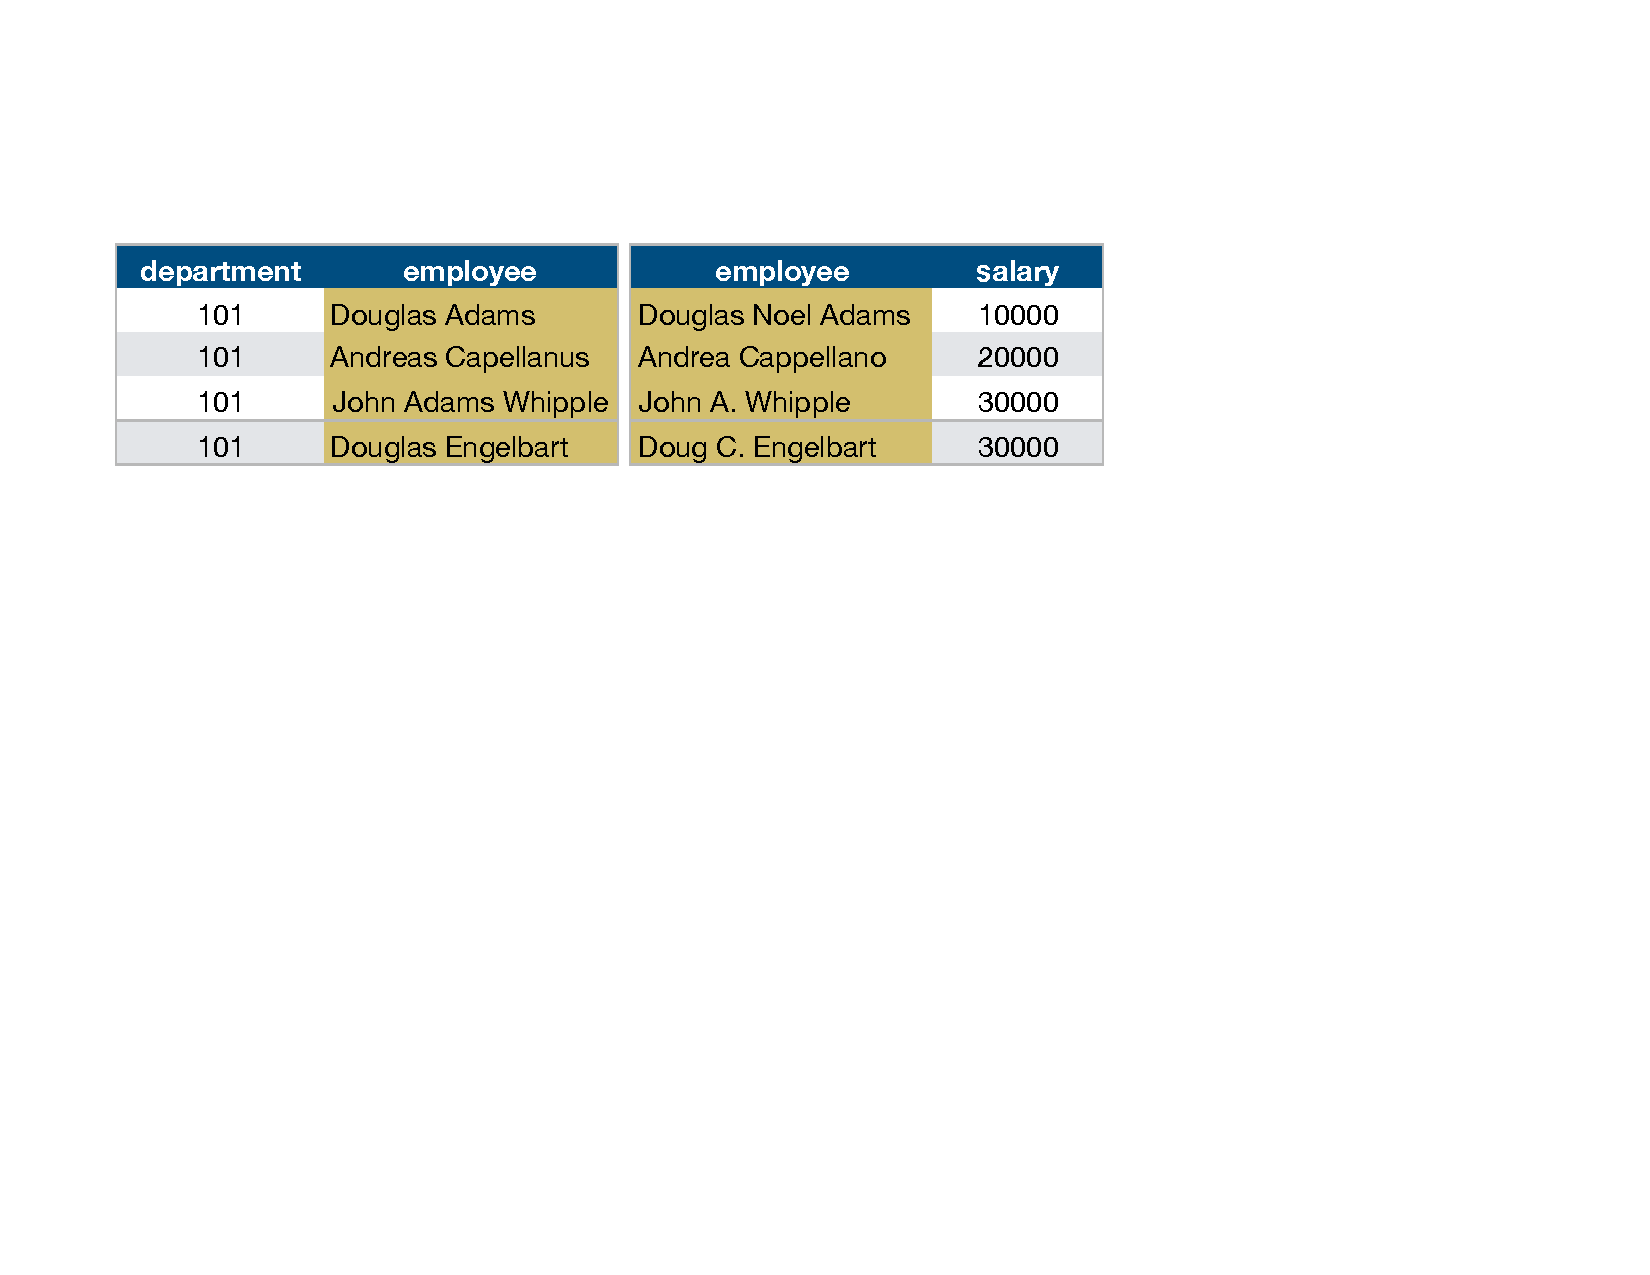
\includegraphics[width=1\linewidth]{fig1}
\label{table-example}
\caption{Example of a join problem}
\end{figure}


\begin{figure}
\centering
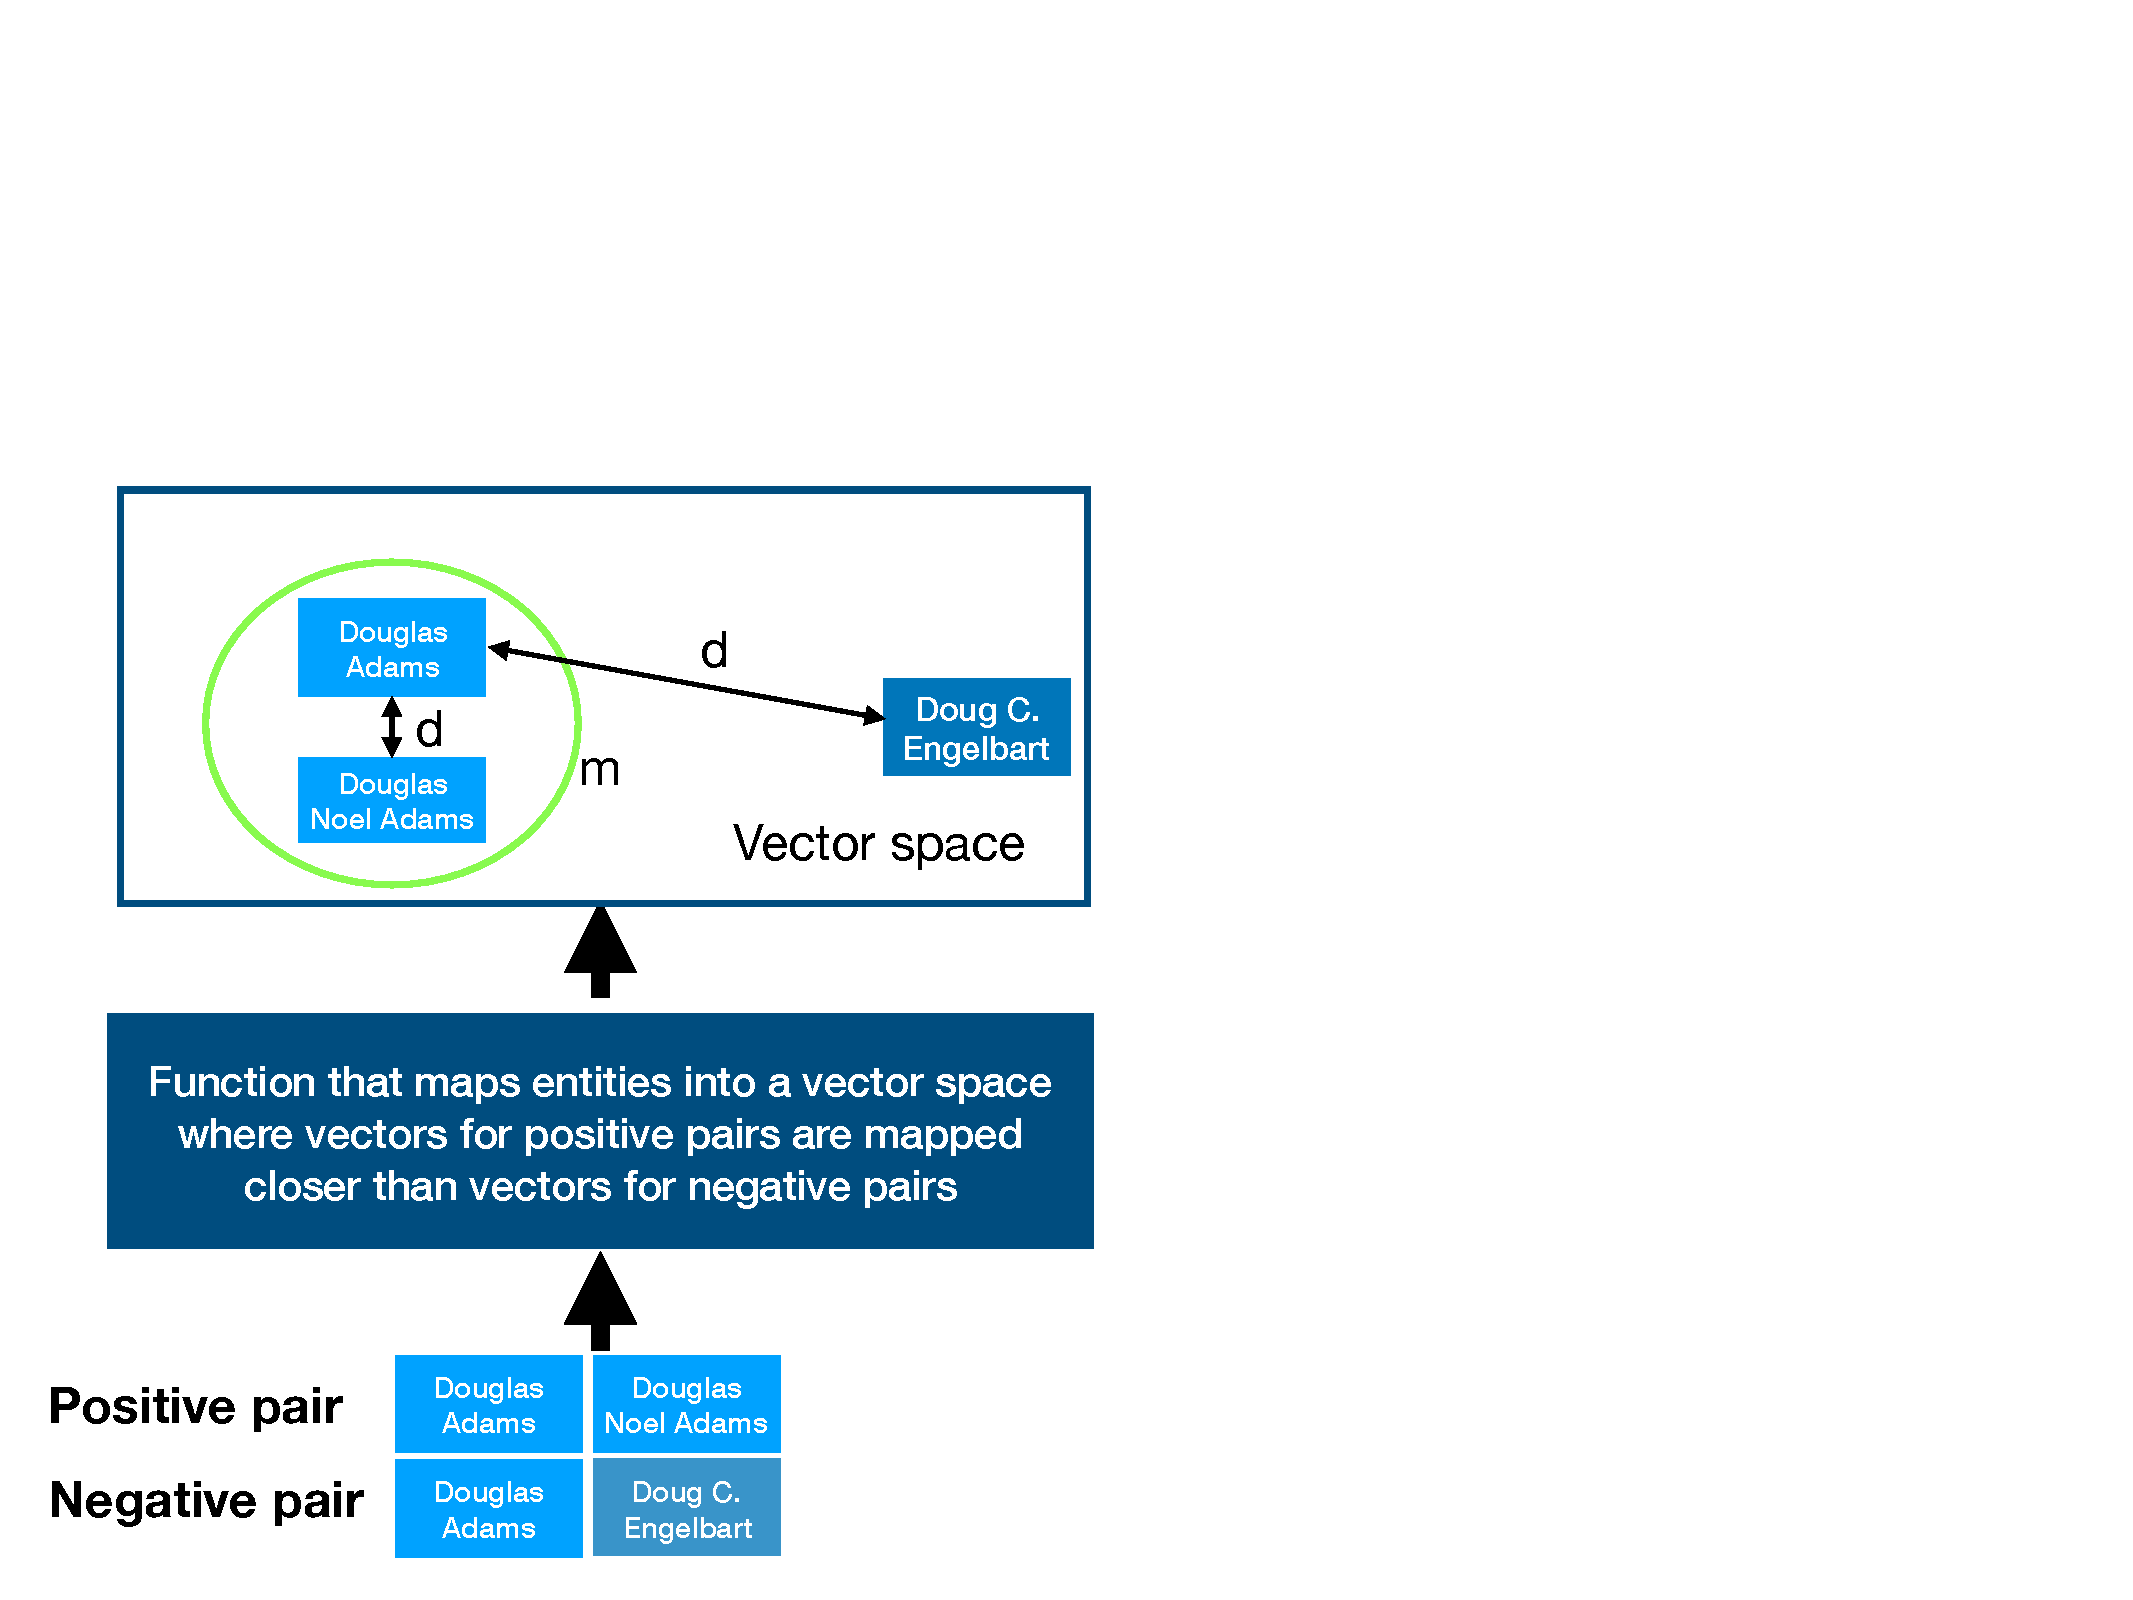
\includegraphics[width=1\linewidth]{fig2}
\label{fig-1}
\caption{Conceptual overview of neural network approach to matching}
\end{figure}

Our key contributions to the join problem are as follows:
\begin{itemize}
\item We demonstrate that we can use a triplet loss network to learn a distance function that successfully discriminates same pairs from different pairs with an accuracy of 97\%.  Our results suggest that deep learning models can be used successfully as another mechanism for data driven joins, assuming some sort of filtering approach has been applied to the data.
\item We try to extend this further; to see if the output of the function can in fact be used in an approximate nearest neighbor algorithm to identify neighbors to match with, without any filtering. 
\end{itemize}


\section{Related Works}
There have been a number of attempts to solve the fuzzy join problem. Many of the attempts use various string matching algorithms for example \cite{Wang:String}. The main issue with using string matching comparisons is that they do not work across a wide variety of entities. To our knowledge no serious machine learning approach has been used for this problem. The problem of blocking has also been dealt with using MapReduce \cite{Vernica:MapReduce}. This approach requires a lot of computing power and, since they use a string matching approach in the end, is hard to generalize across many types of entities. There has also been work done on a related yet different problem of fuzzy joining on whole rows \cite{he_ganjam_chu_2015}. We deal with the case where we only have one column of information.
\section{Algorithm}
\subsection{Rule Based}
We started our process with a simple rule based method for matching and another one for blocking. 


\begin{table*}
\centering
\caption{Table 2}
\begin{tabular}{|c|c|} \hline
Bucket Name&Contents\\ \hline
A&\{John A. Whipple\} \\ \hline
Adams&\{Douglas Adams, Douglas Noel Adams, John Adams Whipple\} \\ \hline
Andreas&\{Andreas Capellanus\} \\ \hline
Andrea&\{Andrea Cappellano\} \\ \hline
Cappellano&\{Andrea Cappellano\} \\ \hline
Capellanus&\{Andreas Capellanus\} \\ \hline
Douglas&\{Douglas Adams, Douglas Noel Adams\} \\ \hline
John&\{John Adams Whipple, John A. Whipple\} \\ \hline
Noel&\{Douglas Noel Adams\} \\ \hline
Whipple&\{John Adams Whipple, John A. Whipple\} \\
\hline
\label{word_table}
\end{tabular}
\end{table*}

In the rule-based method, we block based on items that have one word in common. This is the simplest reasonable blocking strategy. Table \ref{word_table} illustrates what the blocking of the three names from Figure \ref{table-example} would look like. To perform the actual matching, we used three simple rules see Table 3:
\begin{enumerate}

\item If a word is unique to two items, we match them. (`John Adams Whipple' matches `John A. Whipple' since `Whipple' only apears in those two names)
\item If, when all spaces are removed, one of the items is a substring of the other, we match them. (`the flower company' matches `theflowercompany.com' since `theflowercompany' is a subset of `theflowercompany.com')
\item If we treat each name as a set of words, and one set is a subset of the other set, we match them. (`Douglas Adams' matches `Douglas Noel Adams' since \{`Douglas', `Adams'\} $\subseteq$ \{`Douglas', `Noel', `Adams'\})

\end{enumerate} 
Even using these three rules in combination resulted in too many false negatives. Therefore we decided to treat all matches resulting from any of the three rules as valid.
\subsection{Dimensionality Reduction by Learning an Invariant Mapping}

The problem of dimensionality reduction, mapping a high dimensional group of entities onto a low dimensional manifold, is an important problem in many areas of machine learning. Dimensionality Reduction by Learning an Invariant Mapping is a technique for solving this problem by mapping points onto the manifold using a set of previously known matches and non-matches described by \cite{Hasdell:Siamese}. The goal of this technique is to minimize the distance between matched pairs and maximize the distance between unmatched pairs. This is accomplished using a network architecture know as a \textit{siamese} network. In this architecture there are two deep neural networks that share weights attached to a final layer that determines the distance between the output of the two hidden networks and minimizes the loss function. To train the network a set of matched and non-matched pairs of inputs is sent through the network and the weights are adjusted to maximize or minimize distance accordingly.

By mapping the inputs onto meaningful locations on a manifold, this method clusters similar inputs close to each other. Using this property we can use the distance layer to decide if two inputs are matched. We simply set a limit for euclidean distance and match if the outputs of the hidden layers are within that limit, as in Figure \ref{siamese}. This lets us use this method for our problem of matching, we treat items as similar to each other if they are aliases for the same entity and different otherwise. To begin with we created the non-matched pairs by choosing other entities with at least one word in common, to avoid the network learning a useless function. This successfully brought the matches close together in the input but failed to properly distance pairs that should be different, as shown in Figure \ref{comp_dif_fail}. Since we never fed the network pairs that were completely different it did not learn to distinguish them from matches. To combat this we created two types of different pairs: ones that share at least one word in common and ones that are completely different.

\begin{figure}
\centering
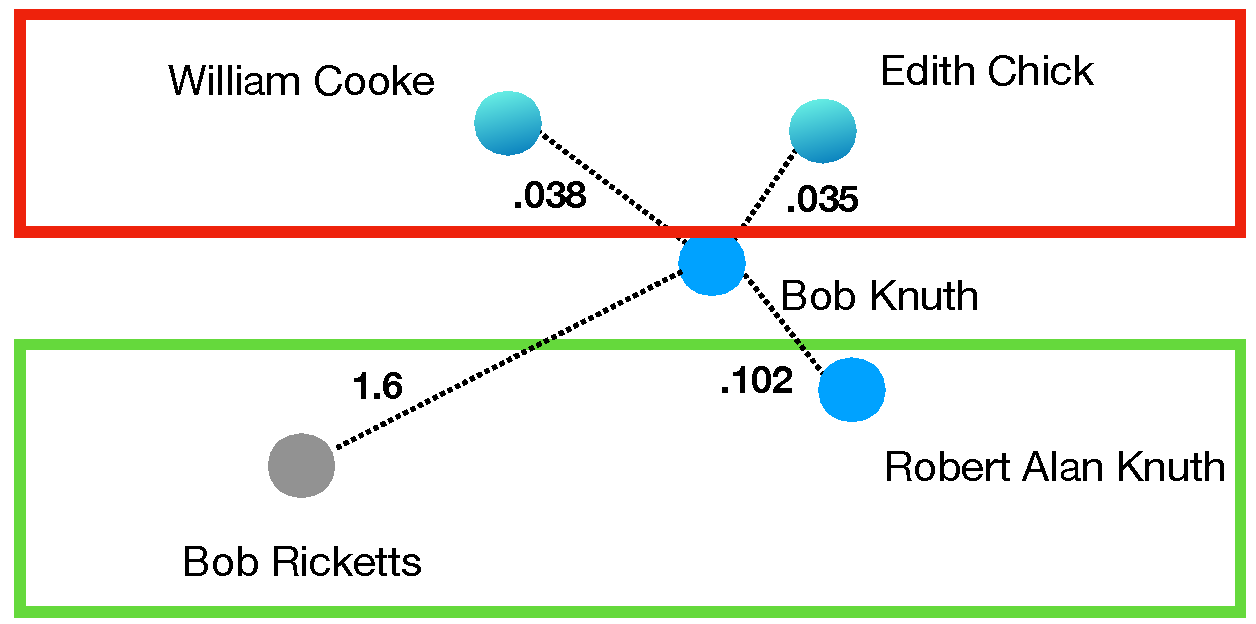
\includegraphics[width=1\linewidth]{word_in_common}
\caption{The model preformed well on somewhat similar names and badly on completely different names}
\label{comp_dif_fail}
\end{figure}
\begin{figure}
\centering
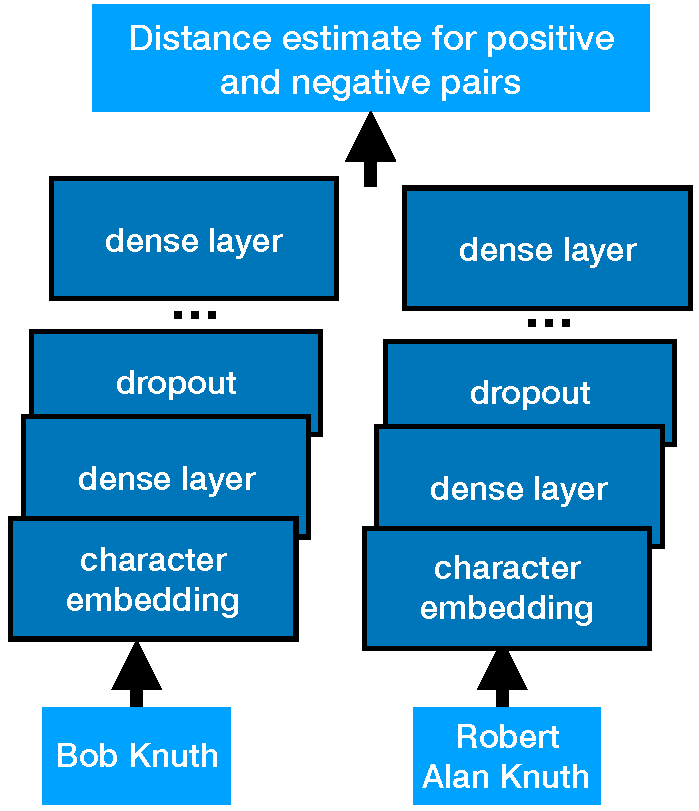
\includegraphics[width=0.5\linewidth]{siamese_arc}
\caption{A siamese network has two networks which share weights which feed into a distance estimator}
\label{siamese}
\end{figure}

\subsection{Approximate Nearest Neighbors}
We used the ANNOY package to find the nearest neighbors in output of the hidden layer computed in the previous section.\cite{annoy_impl} This package approximates the nearest neighbors by first calculating binary trees using the randomized k-d forest method.\cite{ann_paper} These trees are calculated by splitting the vector space by drawing random hyperplanes. Each side of the hyperplane is one node of the binary tree. The algorithm then continues to split each subspace recursively until no more than a predetermined number of items are in each subsection. Some of the neighbors can be found by looking at the items in the same subspace, or subspaces near the target item in the tree. The processes of building a tree is repeated a number of times. By taking a union of the points from all the trees, a reasonable neighborhood is approximated. Once we have a neighborhood of points, we can calculate distance and sort the subset of points. Since much of the time goes into creating the trees, queries can be executed quickly, in logarithmic time.

\subsection{Triplet Loss}
While the previos aproach maps 2 entities at a time using 2 networks that share weights, this aproach maps 3 entities at a time with 3 networks: the anchor the positive and the negative. The loss function minimizes the difference between the anchor and the positive at the same time as it maximises the difference between the anchor and the negative. By doing this we can deal with an unmatched pair and a matched pair at the same time: the anchor is one name, the positive is a match for that name and the negative is another name which is not a match.\cite{schroff2015facenet} We accomplish this by minimizing the following loss function: \[ L(\vec{X}_a, \vec{X}_n, \vec{X}_p) = |\:||\vec{X}_a - \vec{X}_p||^2 - ||\vec{X}_a - \vec{X}_n||^2 + \alpha|\] where $\vec{X}_a$, $\vec{X}_n$, $\vec{X}_p$ are the embedded anchor, negative and positive vectors and $\alpha$ is a constant margin. The key choice here is which vectors to include in the training set. If too many easy triplets are including it will slow down the learning since the constraint will be easily satisfied. If too many hard triplets are included the network will learn a strange function based on unusual cases 

\subsection{LSTM}
A regular Deep Neural network would treat the name like a bag of words, without accounting for order. We experimented with using an LSTM architecture to account for order the words apear in. This makes sense for our use case since first name and last names are different from eachother. In the implimentation we used GRUs (Gated Recurrent Unit), which function like LSTMs but are computationally cheaper.
\section{Experiments}
\subsection{Rule Based}
To test the rule based matcher we ran the blocker followed by the matcher and calculated F-scores based on how many correct matches were in the top 3. We got an F-score of 0.6. Since the issue is mostly false negatives, and therefore even some of the first three slots were often empty, so even if we accept any of the top 1000 as a success, we get an F-score of 0.63, not much better.
\subsection{Siamese Network}
Our first experiment was using a Siamese network to match already blocked entities. The architecture of the network was as shown in Figure \ref{siamese}. As described above this involves two networks that share weights mapping the inputs onto a vector space and computing distance. Before feeding the entities into the networks, we used Kazuma character embeddings to encode each entity as a vector. We used character level embeddings since many names would not have been represented at all if we had used word level embeddings. We then trained the network on our 182772 pairs of names pulled from DBpedia. These are the pairs we have after running the data through the cleanser. We used 95\% of them for training and withheld 5\% for testing. In addition to these pairs we created an equal number of negative pairs to train the model. Wherever possible, the negative pairs had at least one word in common with each other. This was done so that the model would not just learn the obvious function of reject unrelated pairs. We trained the model in 10 epochs. We found that the fscore on the training data was .89 on the test data. This showed that this architecture is an effective matcher. However we only successfully included the correct match in around 15\% of pairs in the top five. This was barely better than the 5\% we got from the embedding alone.
\subsection{Triplet Loss}
The triplet loss experiment was extremely similar to the Siamese one, only we used the Triplet loss network instead of the Siamese one. We used a margin of 1. We also used a GRU instead of a regular deep neural network to capture the order of the words. The last change we used was in selection of negative points, instead of picking them based on some rule, we picked the closest 40 points that were not matches from the character embedding. We did this since those names are the hardest ones for the model to learn, this also avoids the problem in Figure \ref{comp_dif_fail}. When we did this we got 69\% of the items in the top 40. This is a relatively effective blocker. It also correctly placed 97\% of positives closer to the anchor than negatives, making it a very effective matcher.
\section{Conclusions}
While we have a very good machine learning based matcher, that does not appear to translate into very good blocking. We still need to explore why we only getting around 69\% of the matches in the top 40 items, when we have the positive closer than the negative in 97\% of cases.  
%\end{document}  % This is where a 'short' article might terminate

% ensure same length columns on last page (might need two sub-sequent latex runs)
\balance

%ACKNOWLEDGMENTS are optional

% The following two commands are all you need in the
% initial runs of your .tex file to
% produce the bibliography for the citations in your paper.
\bibliographystyle{abbrv}
\bibliography{paper}  % vldb_sample.bib is the name of the Bibliography in this case
% You must have a proper ".bib" file
%  and remember to run:
% latex bibtex latex latex
% to resolve all references

% ****************** APPENDIX **************************************

% Example of an appendix; typically would start on a new page
%pagebreak


\end{document}
